\documentclass[12pt, twoside]{article}
\usepackage[letterpaper, margin=1in, headsep=0.5in]{geometry}
\usepackage[english]{babel}
\usepackage[utf8]{inputenc}
\usepackage{amsmath}
\usepackage{amsfonts}
\usepackage{amssymb}
\usepackage{tikz}
%\usetikzlibrary{quotes, angles}

\usepackage{graphicx}
\usepackage{enumitem}
\usepackage{multicol}

\usepackage{fancyhdr}
\pagestyle{fancy}
\fancyhf{}
\renewcommand{\headrulewidth}{0pt} % disable the underline of the header

\fancyhead[RE]{\thepage}
\fancyhead[RO]{\thepage \\ Name: \hspace{3cm}}
\fancyhead[L]{BECA / Dr. Huson / 10th Grade Geometry\\* Unit 8 Transformations\\19 March 2019}

\begin{document}
\subsubsection*{8-12 Do Now: Regents Geometric Situations}
  \begin{enumerate}

  \item After a dilation with center $(0,0)$, the image of $\overline{MN}$ is $\overline{M'N'}$. If $MN=4.5$ and $M'N'=18$, find the scale factor of this dilation. \vspace{3cm}

  \item In the diagram below, $\triangle ABC$ with sides of 13, 15, and 16, is mapped onto $\triangle DEF$ after a clockwise rotation of $90^\circ$ about point $P$.
      \begin{center}
        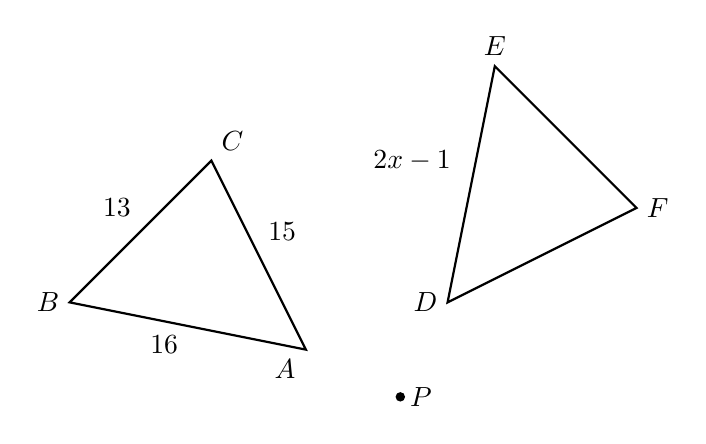
\begin{tikzpicture}[scale=.6]
        %\draw [thick, <->] (-7.4,0) -- (10.4,0) node [right] {$x$};
        %draw [thick, <->] (0,-5.4)--(0,10.4) node [above] {$y$};
        \fill (0,0) circle[radius=0.1] node[right]{$P$};
          \draw [thick]
          (-2,1) node[below left] {$A$}--
          (-7,2) node[left] {$B$}--
          (-4,5) node[above right] {$C$}--cycle;
            \node at (-5,1.5)[below]{16};
            \node at (-6,4){13};
            \node at (-2.5,3.5){15};
            \node at (0.25,5){$2x-1$};
          \draw [thick]
          (1,2) node[left] {$D$}--
          (2,7) node[above] {$E$}--
          (5,4) node[right] {$F$}--cycle;
        \end{tikzpicture}
      \end{center}
    If $DE=2x-1$, what is the value of $x$? \vspace{2cm}

    \item The figure shows a rhombus with noncongruent diagonals.
      \begin{center}
        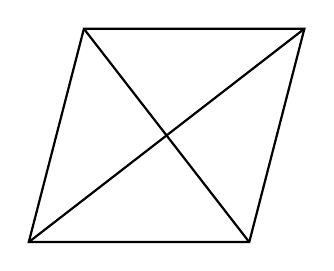
\begin{tikzpicture}[scale=0.7]
          \coordinate (A) at (0, 0); %[label=above left:$P$]
          \coordinate (B) at (4, 0);
          \coordinate (C) at (5, 3.87);
          \coordinate (D) at (1, 3.87);
          \draw [thick] (A)--(B)--(C)--(D)--cycle;
          \draw [thick] (A)--(C);
          \draw [thick] (B)--(D);
          %\draw [thick, xshift=2cm, yshift=2.5cm] (85:3);
        \end{tikzpicture}
      \end{center}
    Which transformations carries the rhombus onto itself? Mark each True or False.
      \begin{enumerate}
        \item A reflection over the shorter diagonal \hfill True \quad False
        \item A reflection over the longer diagonal \hfill True \quad False
        \item A clockwise rotation of $90^\circ$ about the intersection of the diagonals \hfill True \quad False
        \item A clockwise rotation of $180^\circ$ about the intersection of the diagonals \hfill True \quad False
      \end{enumerate}
\newpage
    \item In right triangle $ABC$ shown below, point $D$ is on $\overline{AB}$ and point $E$ is on $\overline{BC}$ such that $\overline{AC} \parallel \overline{DE}$
      \begin{center}
        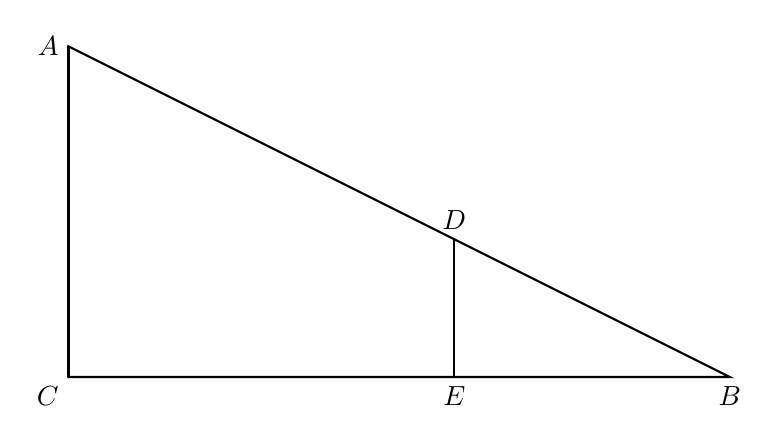
\begin{tikzpicture}[scale=0.7]
          \coordinate [label=left:$A$](A) at (-12,6);
          \coordinate [label=below:$B$](B) at (0, 0);
          \coordinate [label=below left:$C$](C) at (-12,0);
          \coordinate [label=above:$D$](D) at (-5, 2.5);
          \coordinate [label=below:$E$](E) at (-5,0);
          \draw [thick] (A)--(B)--(C)--cycle;
          \draw [thick] (A)--(C);
          \draw [thick] (D)--(E);
        \end{tikzpicture}
      \end{center}
    If $AB=15$, $BC=12$, and $EC=7$, what is the length of $\overline{BD}$?


      \item \emph{Spicy} On the set of axes below, $\triangle ABC$ has vertices at $A(-2,0)$, $B(2,4)$, $C(4,-2)$, and $\triangle DEF$ has vertices at $D(4,0)$, $E(-4,8)$, $F(-8,-4)$.
        \begin{center}
          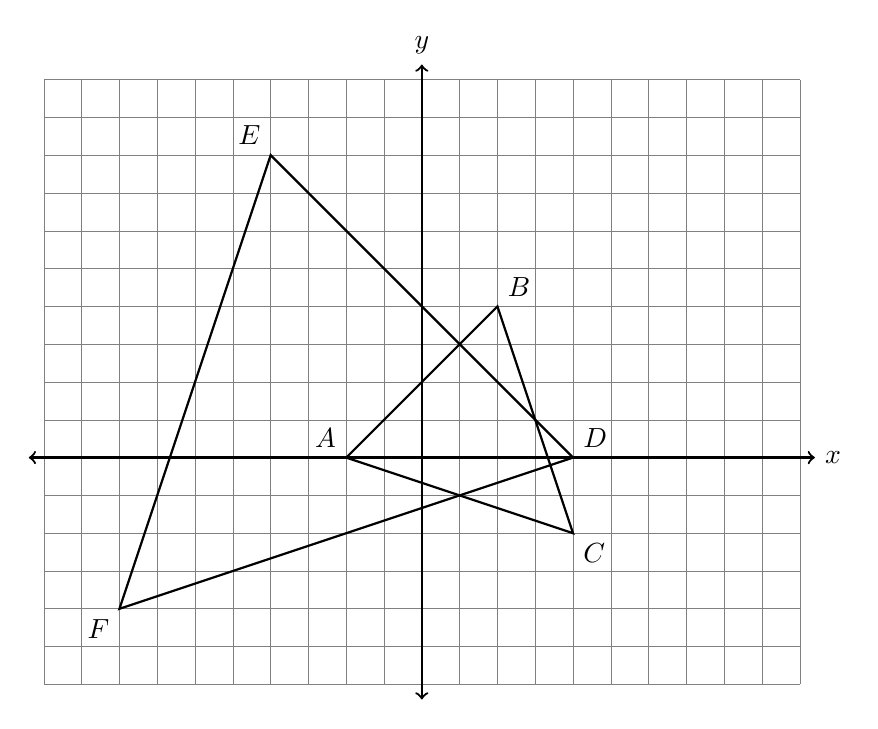
\begin{tikzpicture}[scale=.48]
            \draw [help lines] (-10,-6) grid (10,10);
            \draw [thick, <->] (-10.4,0) -- (10.4,0) node [right] {$x$};
            \draw [thick, <->] (0,-6.4)--(0,10.4) node [above] {$y$};
            \draw [thick]
              (-2,0) node[above left] {$A$}--
              (2,4) node[above right] {$B$}--
              (4,-2) node[below right] {$C$}--cycle;
            \draw [thick]
              (4,0) node[above right] {$D$}--
              (-4,8) node[above left] {$E$}--
              (-8,-4) node[below left] {$F$}--cycle;
          \end{tikzpicture}
        \end{center}
        Which tranformations map $\triangle ABC \rightarrow \triangle DEF$? Mark each statement True or False
          \begin{enumerate}
            \item A dilation with a scale factor of $-2$ centered at the origin \hfill True \quad False
            \item A dilation with a scale factor of $\frac{1}{2}$ centered at point $A$ \hfill True \quad False
            \item A dilation with a scale factor of 2 centered at the origin, followed by a rotation of $180^\circ$ about the origin \hfill True \quad False
            \item A dilation with a scale factor of 2 centered at the origin, followed by a reflection across the $y$-axis \hfill True \quad False
          \end{enumerate}

  \end{enumerate}

  \end{document}
